\documentclass[12pt]{article}

% packages
% -------------------
\usepackage[danish]{babel}
\usepackage[framemethod=TikZ]{mdframed}
\usepackage[utf8]{inputenc}
\usepackage{amsmath}
\usepackage{csquotes}% Recommended
\usepackage{varwidth}
\usepackage{verbatim}
\usepackage{url}
\usepackage{physics}
\usepackage{mathtools}% Loads amsmath
\usepackage{amsmath}
\usepackage{graphicx}

%\usepackage{tgbonum}
%\usepackage{newtxmath}

\usepackage[utf8]{inputenc}
\usepackage{siunitx}
\usepackage{amssymb}
\usepackage{accents}
\usepackage{tikz}
\usetikzlibrary{trees}
\usepackage[danish]{babel}
%\usepackage[margin=4cm]{geometry}

\newcommand{\tss}[1]{\textsubscript{#1}}
\renewcommand{\d}{\mathrm{d}}
\usepackage[scr=boondoxo]{mathalfa}
% -------------------
% siunitx setup
% -------------------
\sisetup{exponent-product = \cdot}
\newcommand{\s}[1]{~\si{#1}}
\newcommand{\us}[1]{~\si{\qty[#1]}}
\newcommand{\kg}{\s{kg}}
\newcommand{\sek}{\s{s}}
\newcommand{\met}{\s{m}}
\newcommand{\metps}{\s{\frac{m}{s}}}
\newcommand{\newt}{\s{N}}
\newcommand{\hz}{\s{hz}}
\newcommand{\radia}{\s{rad}}

% -------------------
% centerverbatim
% -------------------
\newenvironment{centerverbatim}{%
  \par
  \centering
  \varwidth{\linewidth}%
  \verbatim
}{%
  \endverbatim
  \endvarwidth
  \par
}

\usepackage[explicit]{titlesec}

% -------------------

% -------------------
\usepackage[style=authoryear-ibid,backend=biber]{biblatex}
\bibliography{sample.bib}

% -------------------
% custom env
% -------------------
\usepackage{amsthm}
%\newtheorem{theorem}{Theorem}
\newtheorem{theorem}{Theorem}[subsection]
\newtheorem{corollary}{Korollar}[theorem]
\theoremstyle{definition}
\newtheorem{example}{Eksempel}[definition]
\newtheorem{lemma}[theorem]{Lemma}
\theoremstyle{remark}
\newtheorem*{remark}{Note}
\theoremstyle{definition}
\newtheorem{definition}{Definition}[section]
\renewcommand\qedsymbol{$\blacksquare$}
%

\addbibresource{sample.bib}% Syntax for version >= 1.2
\usepackage[style=authoryear-ibid,backend=biber]{biblatex}


% -------------------
% texthøjde
% -------------------
\usepackage{setspace}
\renewcommand{\baselinestretch}{1.5}
\renewcommand{\H}{\mathcal H}
\renewcommand{\arraystretch}{0.5}
%\linespread{1.5}

% -------------------
% box
% -------------------
\newcounter{theo}[section]\setcounter{theo}{0}
\renewcommand{\thetheo}{\arabic{section}.\arabic{theo}}
\newenvironment{theo}[2][]{%
  \refstepcounter{theo}%
  \ifstrempty{#1}%
  {\mdfsetup{%
      frametitle={%
        \tikz[baseline=(current bounding box.east),outer sep=0pt]
        \node[anchor=east,rectangle,fill=blue!20]
        {\strut #2};}}
  }%
  {\mdfsetup{%
      frametitle={%
        \tikz[baseline=(current bounding box.east),outer sep=0pt]
        \node[anchor=east,rectangle,fill=blue!20]
        {\strut Theorem~\thetheo:~#1};}}%
  }%
  \mdfsetup{innertopmargin=10pt,linecolor=blue!20,%
    linewidth=2pt,topline=true,%
    frametitleaboveskip=\dimexpr-\ht\strutbox\relax
  }
  \begin{mdframed}[]\relax%
    \label{#2}}{\end{mdframed}}

% -------------------
% parindent
% -------------------
\parindent{\noindent}
\usepackage{blindtext}
% -------------------
% titlepage
% -------------------
\title{
  {{Teoretisk bestemmelse af energiniveauer i hyrogenlignende atom}}\\
  {\large{Louis Clément, 3.i}}\\
  {\large Hillerød Tekniske Skole}\\
  \vspace{2cm}
  {
\includegraphics[scale=1.5]{gym.png}}
  \vspace*{1.5cm}
}
\author{
  \begin{tabular}[!h]{c}
    \textbf{Område}\\
                Matematik A, Fysik A \\
    \textbf{Vejledere}\\
                 Mikkel Oglesby \\ Jacob Skytte Salgaard Bendtsen
  \end{tabular}
}
\date{\vspace*{1cm}{18. december 2020}}

%\titleformat{\section}{\huge\textbf}{\titlebar{3em}{\thesection}}{0.1cm}{#1} \titleformat{\subsection}{\large\textbf}{\titlebar{5em}{\thesubsection}}{0.1cm}{#1}
\usepackage{atbegshi}% http://ctan.org/pkg/atbegshi
\AtBeginDocument{\AtBeginShipoutNext{\AtBeginShipoutDiscard}}
\numberwithin{equation}{section}

\begin{document}


\pagenumbering{gobble}
\maketitle
\newpage
\begin{abstract}
\noindent 
    Jeg undersøger en teoretisk kvantemekanisk model for Hydrogenlignende atomer, og sammenligner den med den empiriske Rydbergformel, for til slut at udlede spektrumlinjer på et hydrogenlampespektrum.
\end{abstract}

\tableofcontents

\newpage
\setcounter{page}{1}
\pagenumbering{arabic}

\section{Introduktion}
\subsection{Opgaveformulering}
Hovedspørgsmålet lyder
\begin{quote}
    Teoretiskbestemmelse af energiniveauer i et hydrogenlignende atom
\end{quote}
Dertil en række arbejdsspørgsmål
\begin{itemize}
    \item Redegør for Schrödinger-ligningen
    \item Redegør for de matematiske begreber og metoder, der ligger bag Schrödinger-ligningen, og løsningen af denne
    \item Løs Schrödinger-ligningen for en partikel i en en-dimensionaluendelige potentialbrønd.
    \item Bestem energiniveauerne for et hydrogenlignende atom
    \item Analyser og perspektiverde teoretiske energiniveauer,til eksperimentelle værdier og/eller tabelværdier for hydrogens spektrum.
    \end{itemize}

\section{Gennemgang af matematiske metoder}
\subsection{Hilbertrum}

\begin{definition}
  Et Hilbertrum $\mathcal H$ er et komplet vektorrum over et felt $\mathbb F$ med associeret indre produkt. Vi beskæftiger os med rum, hvori det gælder at
  \begin{align}
   \label{l2}
    \braket{\psi}{\psi} = \int_{\mathbb F} \psi^*(x)\psi(x) ~ dx < \infty
  \end{align}
  for $\ket \psi \in \mathcal H$. Denne betingelse gør $\psi$ til en del af $L^2(\mathbb F)$ rum, og gælder for $\mathbb R$ eller $\mathbb C$. Vi kan konstruere et $\infty$-dimensionelt Hilbertrum ved at overveje et kontinuert basis med elementerne $\ket a$ navngivet med en kontinuer variabel $a$, normaliseret således at
  \begin{align}
    \label{eq:con}
    \braket{a}{\tilde a} = \delta(a-\tilde a)
  \end{align}
  hvilket betyder vi kan skrive
  \begin{align}
    \label{eq:sw}
    \ket \psi = \int \psi(a)\ket a~da
  \end{align}
  
\end{definition}


\begin{definition}
  En \textit{ket} vektor $\ket V$ betegner en vektor af et abstrakt
vektorrum. I et endeligdimensionelt vektorrum kan en ket vektor
repræsenteres som
  \begin{align}
    \label{eq:colv}
    \ket V \leftrightarrow \mqty[v_1\\v_2\\\vdots\\ v_n]
  \end{align}
\end{definition}

\begin{definition}
  En \textit{bra} vektor $\bra V$ betegner en et element af dual
vektorrum (dualrum). Den kan repræsenteres som det transponerede
konjugat af den ket vektor den er dual på
  \begin{align}
    \label{eq:ket}
    \ket V \leftrightarrow \mqty[v_1\\v_2\\\vdots\\v_n]
\leftrightarrow \mqty[v_1^*&v_2^*&\cdots&v_n^*]
\leftrightarrow \bra V
  \end{align}
  Dualrum $\mathcal H^*$ består af linære afbildninger $\H^*\to \H$,
defineret med det indre produkt for $\langle \phi,\cdot \rangle\in
\H^$ som $\langle \phi,\cdot\rangle : \psi \mapsto
\braket{\phi}{\psi}$.
\end{definition}


\subsection{Linære operatorer}
\begin{definition}
En linær operator $\Omgea$ eller linær transformation $T$ er en
funktion $T:\mathbb V_1 \to \mathbb V_2$ således at
\begin{align}
  \label{eq:2}
  T(cv_1+v_2) = c(Tv_1) + Tv_2
\end{align}
Igennem denne tekst vil de kun repræsenteres som matricer $M$, således
at $T(x)=Mx$. En linær operator kan i øvrigt repræsenteres som $\ket
\psi \bra \phi \in \mathcal H \otimes \mathcal H^*$.

\end{definition}

\begin{definition}
  En kommutator er defineret som
  \begin{align}
    \label{eq:com}
    [\Omega, \Lambda] = \Omega\Lambda - \Lambda \Omega
  \end{align}
  hvor $\Omega,\Lambda \in \H\otimes \H^*$. Hviss. $[\Omega, \Lambda]
= 0$ kommuterer operatorerne.

\end{definition}

\begin{definition}
Enhver operator i $\mathbb V^n(C)$ har $n$
eigenværdier. Eigenværdiligningen (en omskrevet version) er
\begin{align}
  \label{eq:eigen}
  (\Omega - \omega \hat I)\ket V = \ket 0
\end{align}
Betingelsen for eigenvektoren er
\begin{align}
  \label{eq:kre}
  \det(\Omega-\omega \hat I) = 0
\end{align}
hvor $\hat I$ er identitetsoperatoren. Vi kan omskrive
eigenværdiligningen (ved at projicere den på en basis $\bra i$) til
\begin{align}
  \label{eq:eig2}
  \begin{split}
   \bra i \Omega - \omega\hat I \ket V = 0 \\
   \sum_j (\Omega_{ij}-\omega \delta_{ij})v_j = 0 
  \end{split}
\end{align}

Sættes determinanten til 0 får vi karakterligningen 
\begin{align}
  \label{eq:karklig}
  \sum_{m=0}^n c_w \omega^m = 0
\end{align}
og karakterpolynomiet
\begin{align}
  \label{eq:ei}
  P^n(\omega) = \sum_{m=0}^n c_w \omega^m
\end{align}
\end{definition}

\section{Atomfysik og kvantemekaniske principper}
\subsection{}

\subsection{Tilstand}
Tilstanden af et partikel er beskrevet med en tilstandsvektor $\ket
\psi\in \mathcal H$. Alle observerbare kvantiteter har en associeret linær Hermitisk operator, som vi kan bruge i sammenhæng med førnævnte tilstandsvektor. Givet en operator, $\Omega$, kan man kun fysisk observere denne operators egenværdier $\omega$
\begin{align}
    \label{eigenstate}
    \Omega\ket{\psi_i} = \omega_i \ket{\psi_i}
\end{align}
(\ref{eigenstate}) følger af at enhver tilstand kan omskrives til en linær kombination af andre tilstande, som
\begin{align}
    \ket \psi = \sum c_i \psi_i
\end{align}
Efterfølgende en observation, kollapser tilstanden på en givet egentilstand. Det er vigtigt at pointere at de eneste mulige resultater for en given operators $\Omega$ observation, er dens egenværdier.

\subsection{Schrödinger-ligningen}
Schrödinger-ligningen er et postulat om hvordan kvantemekaniske tilstande følger givet information om tilstanden eller dens omstændigheder. Man kan skrive den tidsafhængige Schrödinger-ligning (TDSE) som
\begin{align}
  \label{eq:schr}
  \hat H \ket{\psi(t)} = i\hbar \partial_t \ket{\psi(t)}
\end{align}
Hvor $\hat H$ er Hamiltonoperatoren. 
I positionsrum vil tilstandsvektoren udtrykkes i en basis bestående af positionsvektoren ${\ket x}$ for $x\in \mathbb R$, som $\braket{x}{\psi}$. Fra (\ref{eq:sw}) får vi 
\begin{align*}
    \ket{\psi} &= \int_{\mathbb R} \psi(\tilde x)\ket{\tilde x}~d\tilde x \\
    \braket{x}{\psi} &= \int_{\mathbb R} \psi(\tilde x)\braket{x}{\tilde x}~d\tilde x \\
    &= \psi(x,t)
\end{align*}
Fra den klassiske formidling af energi kan vi forstå Hamiltonen $H$ som at repræsentere summen af kinetisk $T$ og potentielt energi $V$ i et system som
\begin{align}
    H &= T(p)+V(q)
\end{align}
I næste sektion vil vi bruge denne formidling for et punktpartikel ($x=x(q)$ for gen. koordinat transformation, siden position er den eneste frihedsgrad), hvor det gælder at $p=mv^2$, således at man får
\begin{align}
    H &= \frac{p^2}{2m} + V(x)
\end{align}
I kvanteteori bliver vi nødt til at beskrive disse kvantiteter, $p$ og $x$ (og Hamiltonen sig selv) som observerbare variable vi kan finde ved at anvende deres tilsvarende operator på en tilstand. Dermed får vi
\begin{align}
    \hat H = \frac{\hat p^2}{2m}+V(\hat x)
\end{align}

\newpage
\section{1-dimensionel uendelig partkelbrønd}
\begin{figure}[!h]
    \centering
    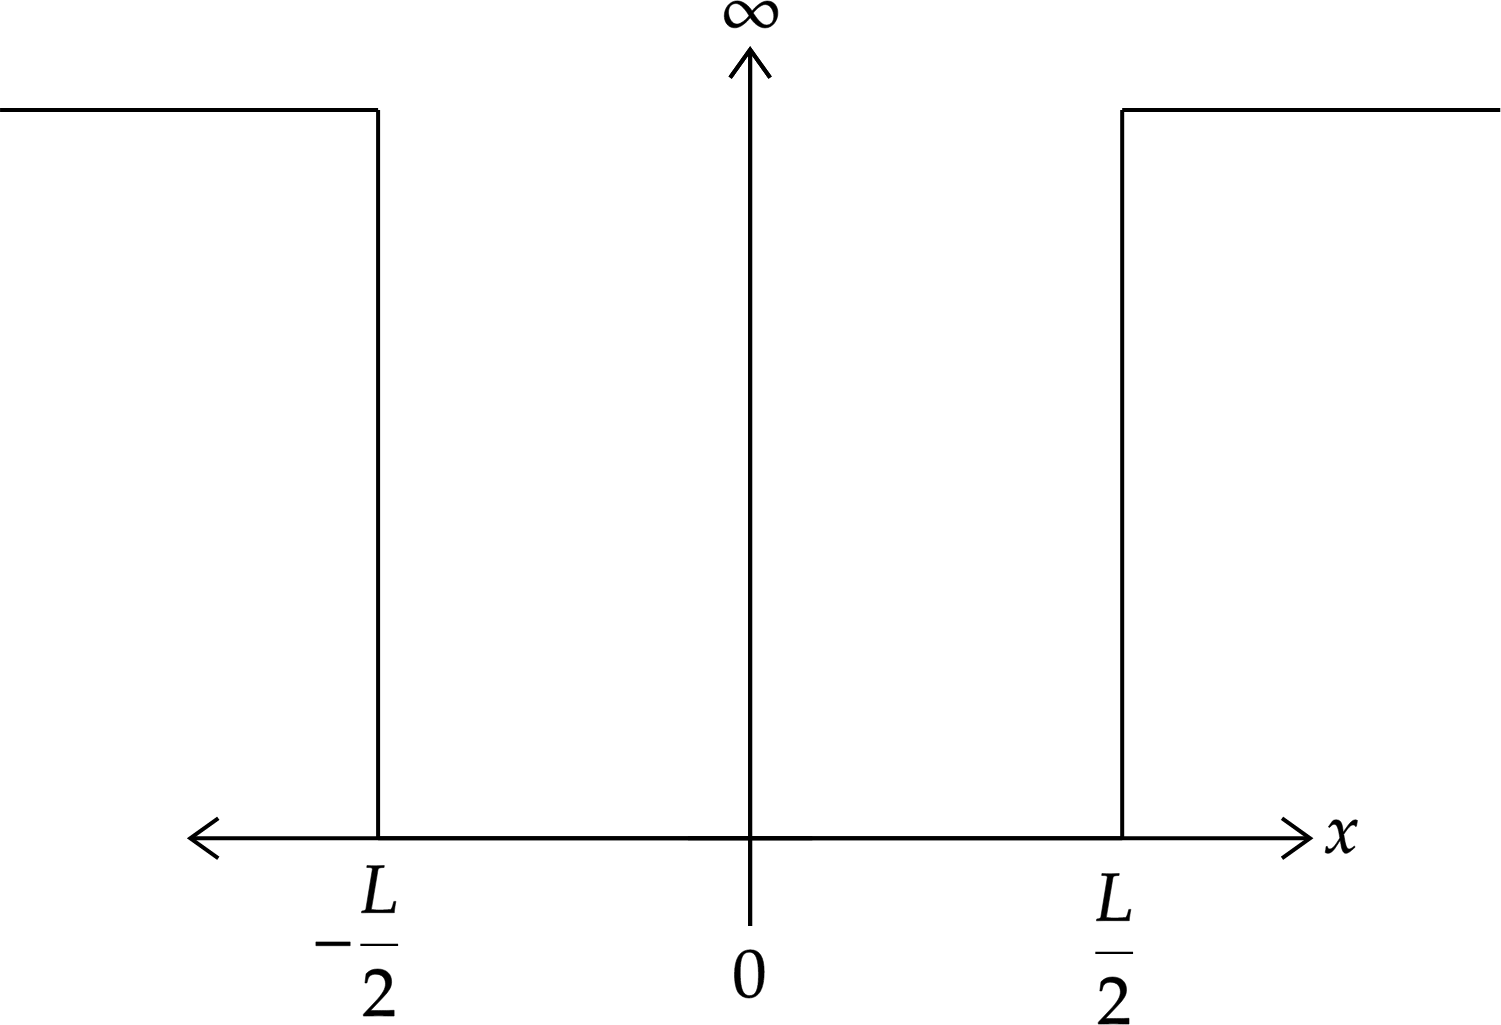
\includegraphics[scale=0.16]{diagram-20201209.png}
    \caption{$V(x)$ potentialet}
    \label{fig:pot1}
\end{figure}
Vi begynder med en beskrivelse af et 1-dimensionelt potentiale $V(x)$ som set på Figur \ref{fig:pot1}. Potentialet er $\infty$ udenfor længden $L$, samt 0 indenfor, heraf navnet ``partikelbrønd''. Dette kan beskrives således
\begin{align}
    V(x) = \begin{cases}
    0, & -\frac{L}{2} < x < \frac{L}{2} \\
    \infty, & x \leq -\frac{L}{2} \\
    \infty, & x \geq \frac{L}{2}
    \end{cases}
\end{align}
I en positionsbasis kan vi omskrive TISE fra (\ref{tise}) til
\begin{align}
     \label{awdb}
    \dv[2]{\psi}{x}+\frac{2m}{\hbar}(E-V(x))\psi = 0
\end{align}
Det er oplagt at inddele bølgefunktionen ind i tre regioner per potentialet. Jeg har denoteret bølgefunktionen venstre og højre region i ``væggen'' med hhv. 1 og 3 (ikke at forvirres med kvantetal). Indenfor væggene er bølgefunktionen kaldt $\psi_2$. Siden dette rimeligt kunstige potentiale er uendeligt kan et partikel selvfølgelig ikke befinde sig deri, da får vi at $\psi_1=0$ og $\psi_3=0$. Vi kan vise dette ved at løse (\ref{awdb}), hvori $V(x)$ i regionen sættes til et udefineret $\tilde V>E$, således at vi kan tilnærme os den faktiske $V$ som grænseværdi
\begin{align}
    \overbrace{
    \lim_{\tilde V\rightarrow \infty} \underbrace{\qty[\dv[2]{\psi_1}{x}-\frac{2m}{\hbar^2}(\tilde V-E)\psi_1]}_{\tilde \psi_1}}^{\psi_1} = 0
\end{align}
Denne ligning er en andensorden linær homogen differentialligning. Som set i (X.X), er løsningen for indholdet af parentesen af formen
\begin{align}
    \tilde \psi_1 = Ae^{-kx}+Be^{kx}
\end{align}
Hvor $\displaystyle k = \sqrt{\frac{2m(\tilde V-E)}{\hbar^2}}$. Siden denne region er defineret for $x\leq-\frac{L}{2}$, kræves der at $\psi_1\in L^2(\mathbb R^-)$ som set i (\ref{l2}) for at dette skal repræsentere noget fysisk. Vi kan løse dette ved at sætte $A=0$, da $Ae^{-kx}$ divergerer når $x\to -\infty$, hvorved vi ender med $\tilde \psi_1=Be^{kx}$. Nu kan vi løse grænseværdien som
\begin{align}
    \psi_1 = \lim_{\tilde V\to \infty } Be^{kx} = 0
\end{align}
Lignende kan det omvendte vises for at $\psi_3=0$. Siden $V=0$ for $\psi_2$, kan vi referere til (X.X) for at få en løsning af formen
\begin{align}
\label{mid}
    \psi_2 &= Ae^{ikx}+Be^{-ikx}
\end{align}
Hvor $\displaystyle k = \sqrt{\frac{2mE}{\hbar^2}}$. Den totale bølgefunktion $\psi$ skal selvfølgelig være kontinuer, da kræver vi at
\begin{align}
\label{betingelsea}
    \psi_1\qty(-\frac{L}{2})=\psi_2\qty(-\frac{L}{2})=0
\end{align}
samt at
\begin{align}
    \psi_3\qty(\frac{L}{2})=\psi_2\qty(\frac{L}{2})=0
\end{align}
Vi omskriver (\ref{mid}) til at være
\begin{align}
    \psi_2 = A\cos(kx)+B\sin(kx)
\end{align}
Jeg undersøger nu hvor denne nulfaktor skal komme fra ved $x=+L/2,-L/2$. Antager man at den skal opstå fra $\sin(kx)$ kræves der at $kx=0$ ved f.eks $x=L/2$. Det er muligt såfremt at 
\begin{align}
\label{forstelso}
    k=\frac{n\pi}{L},\quad n=0,~\pm~2,~\pm 4,\dots
\end{align} I dette tilfælde kræves der at $A=0$. Gør vi det samme med $\cos(kx)$ finder man en række løsninger af samme form som (\ref{forstelso}), hvori $n$ er alle ulige naturlige tal. Dette efterlader os med en række løsninger for bølgefunktionen
\begin{align}
    \psi_n = \begin{cases}
    A\sin\qty(\frac{n\pi x}{L}) & n=\pm2,~\pm 4,\dots \\
    B\cos\qty(\frac{n\pi x}{L}) & n=\pm1,~\pm 3,\dots
    \end{cases}
\end{align}
Vi kan kort konkludere at $A=B$, samt finde normaliseringsfaktoren som
\begin{align}
\begin{split}
    \braket{\psi_n}{\psi_n} &= A \int_{-\frac{L}{2}}^{\frac{L}{2}} \sin^2\qty(\frac{n\pi x}{L})~dx=1 \\
    A &= \sqrt{\frac{2}{L}}
\end{split}
\end{align}
Vi kan udlede energiegenværdierne $E_n$ fra relationen
\begin{align}
    k = \sqrt{\frac{2mE_n}{\hbar^2}} &= \frac{n\pi}{L}
\end{align}
da får vi
\begin{align}
    E_n = \frac{\hbar^2}{2m}k^2_n = \frac{\hbar^2\pi^2n^2}{2mL^2}
\end{align}

\section{Hydrogenatomet}
\subsection{Potentialenergi}
Et Hydrogenlignende atom er ethvert atom der består af ét elektron samt et eller flere protoner. Problemet vi undersøger har med at gøre to ladninger, hhv. $-e$ og $+e$, samt to masser $m$ og $M$ som korresponderer til hhv. elektronet og protonet. Den reducerede masse $\mu = \frac{mM}{m+M}$. Fra Coulomb's lov, får man
\begin{align}
    V(r) = \frac{-e^2}{4\pi \epsilon_0 r}
\end{align}
Hvilket beskriver potentialenergien mellem en elektronladning og atomkernen. Den kinetiske energi kan udledes fra den klassiske formalisme i.e.
\begin{align}
    T(q) = \frac{-\hbar^2}{2m}\pdv[2]{q} 
\end{align}
Hvilket giver os
\begin{align}
    T(r) = \frac{-\hbar^2}{2\mu}\nabla^2
\end{align}
Dette udgør nu vores Hamiltonoperator $\hat H = T(r)+V(r)$, og i TISE får vi da
\begin{align}
\label{unextended}
    \qty[\frac{-\hbar^2}{2\mu}\nabla^2 - \frac{-e^2}{4\pi \epsilon_0 r}]\psi(r,\theta,\phi)=E\psi(r,\theta,\phi)
\end{align}
Vi kan repræsentere $\nabla^2$ i sfæriske koordinater fra
\begin{align}
\nabla^2f &= \frac{1}{r^2} \frac{\partial}{\partial r} \left(r^2 \frac{\partial f}{\partial r} \right) + \frac{1}{r^2 \sin \theta} \frac{\partial}{\partial \theta} \left(\sin \theta \frac{\partial f}{\partial \theta} \right) + \frac{1}{r^2 \sin^2 \theta} \frac{\partial^2 f}{\partial \varphi^2},
\end{align}
Hvorfra vi kan omskrive (\ref{unextended}) som
\begin{align}
    \begin{split}
         -\frac{\hbar^2}{2 \mu} \left[ \frac{1}{r^2} \frac{\partial}{\partial r} \left( r^2 \frac{\partial \psi}{\partial r} \right) + \frac{1}{r^2 \sin \theta} \frac{\partial}{\partial \theta} \left( \sin \theta \frac{\partial \psi}{\partial \theta} \right) + \frac{1}{r^2 \sin^2 \theta} \frac{\partial^2 \psi}{\partial \phi^2} \right]\\ - \frac{e^2}{4 \pi \epsilon_0 r} \psi = E \psi
    \end{split}
\end{align}
Vi ønsker, fra separation af variable, at opdele bølgefunktionen som et produkt af 3 funktioner
\begin{align}
    \psi(r, \theta, \phi) = R(r)\Theta (\theta) \Phi (\phi)
\end{align}
\subsection{Spektrum}

\subsection{Analytisk løsning}
\section{Konklusion}

\newpage
\nocite{*}
\printbibliography

\end{document}
